\documentclass[9pt,t,aspectratio=169]{beamer}
\usetheme[white]{Wisconsin}
\usepackage[utf8]{inputenc}
\setbeamertemplate{page number in head/foot}[totalframenumber]
\setbeamerfont{title}{size=\LARGE}
\setbeamerfont{subtitle}{size=\Large}
\setbeamerfont{block body}{size=\footnotesize}
\setbeamerfont{author}{size=\LARGE}
\setbeamerfont{date}{size=\Large}
\setbeamerfont{institute}{size=\large}
\setlength{\leftmargini}{0pt}


\usepackage{caption}
\captionsetup[figure]{labelformat=empty} % turn off labeling caption figures
%subcaptions
\usepackage{subcaption}
\captionsetup[subfigure]{labelformat=empty} % turn off labeling subcaption figures

% turn off Figure in captions
\usepackage{caption}
% \captionsetup[figure]{labelformat=empty}

\newcommand{\QOR}{\qquad \text{OR} \qquad}
\newcommand{\QAND}{\qquad \text{AND} \qquad}
\newcommand{\QTHUS}{\qquad \text{THUS} \qquad}
\newcommand{\QTHEN}{\qquad \text{THEN} \qquad}
\newcommand{\QWITH}{\qquad \text{WITH} \qquad}
\newcommand{\QFOR}{\qquad \text{FOR} \qquad}
\newcommand{\QSO}{\qquad \text{SO} \qquad}
\newcommand{\QWHERE}{\qquad \text{WHERE} \qquad}
\newcommand{\LINE}{\par\noindent\rule{\textwidth}{0.4pt}\par}
\newcommand{\toinf}{\rightarrow\infty}
\newcommand{\tozero}{\rightarrow0}
\newcommand{\qeq}{\overset{?}{=}}
\newcommand{\ceq}{\overset{\checkmark}{=}}
\renewcommand{\epsilon}{\varepsilon}
\newcommand{\keff}{$k_{e\!f\!f}$}
\newcommand{\kinf}{$k_{inf}$}

% table packages
\usepackage{booktabs}

% Roman Numerals
\newcommand{\rom}[1]{\expandafter\uppercase{\Romannumeral #1\relax}}

% hypersetup
\usepackage{hyperref}
\hypersetup{colorlinks,
            linkcolor = black,
            citecolor = black,
            urlcolor = cyan
}


\def\brac#1{\{#1\}}
\def\Brac#1{\big\{#1\big\}}
\def\BRAC#1{\bigg\{#1\bigg\}}
\def\angbrac#1{\langle#1\rangle}
\def\Angbrac#1{\big\langle#1\big\rangle}
\def\ANGBRAC#1{\bigg\langle#1\bigg\rangle}

% Transitional slides between sections
\AtBeginSection[]
{
    \begin{frame}
        \frametitle{Table of Contents}
        \tableofcontents[currentsection]
    \end{frame}
}


% Bibliography
\usepackage[sorting=none]{biblatex} %Imports biblatex package and cites in order of appearance
\addbibresource{physor2024_pres.bib} %Import the bibliography file
% make all font colors white
\setbeamercolor{bibliography item}{fg=black}
\setbeamercolor{bibliography entry author}{fg=black}
\setbeamercolor{bibliography entry title}{fg=black}
\setbeamercolor{bibliography entry location}{fg=black}
\setbeamercolor{bibliography entry note}{fg=black}
% adds numeric labels linked to bib entries
\setbeamertemplate{bibliography item}{\insertbiblabel}

% eliminate header within an environment
\makeatletter
    \newenvironment{withoutheadline}{
       \setbeamertemplate{headline}[default]
       \def\beamer@entrycode{\vspace*{-\headheight}}
    }{}
\makeatother

% appendix renumbering
\usepackage{appendixnumberbeamer}
% frame breaks with same title
\setbeamertemplate{frametitle continuation}[from second][]

\title{Exploring Effects of Homogenization on an OpenMC Depletion Analysis}
\subtitle{of a TRISO Fueled, Helium Cooled Microreactor}
\author{\vspace*{-0.45cm}Lewis I. Gross\textsuperscript{1}, Patrick Shriwise\textsuperscript{2,1}, Benjamin Lindley\textsuperscript{1} and Paul P.H. Wilson\textsuperscript{1}}
\institute{University of Wisconsin-Madison\textsuperscript{1}, Argonne National Lab\textsuperscript{2} }
\date{\vspace*{-0.25cm}April 24, 2024}
%%----------------------------------------------------------------------------%%
\begin{document}

\begin{withoutheadline}
\begin{frame}[plain] % the plain makes the first frame look good
    \maketitle
\end{frame}
\end{withoutheadline}

\author{Lewis Gross, Patrick Shriwise, Ben Lindley, and Paul Wilson} % reset author so affiliations don't show up in footer
%%----------------------------------------------------------------------------%%
%% Overview
%%----------------------------------------------------------------------------%%
\begin{withoutheadline}
\begin{frame}{Outline}
  \tableofcontents
\end{frame}
\end{withoutheadline}


%%----------------------------------------------------------------------------%%
%% Section 1
%%----------------------------------------------------------------------------%%
\section{Virtual Test Bed Gas-Cooled Microreactor}
\hypersetup{citecolor=white}
\begin{frame}{Microreactors \cite{INL_MR}}
    \begin{figure}
        \centering
        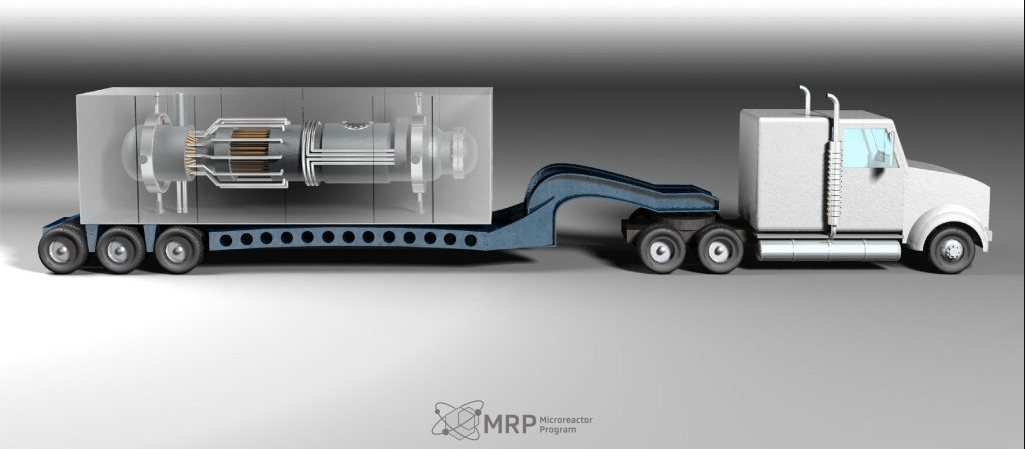
\includegraphics[width=0.95\linewidth]{figures/INL_MR.png}
    \end{figure}
\end{frame}

\begin{frame}{Virtual Test Bed \cite{vtb2023}}
    \begin{figure}
        \centering
        
\includegraphics[width=0.65\linewidth]{figures/nric_logo.png}
    \end{figure}
    \begin{figure}
        \centering
        
\includegraphics[width=0.6\linewidth]{figures/NEAMS.png}
    \end{figure}
\end{frame}
\hypersetup{citecolor=black}

\begin{frame}{TRISO Fuel Particles}
    \begin{minipage}[t]{0.45\linewidth}
        \begin{figure}
            \centering
            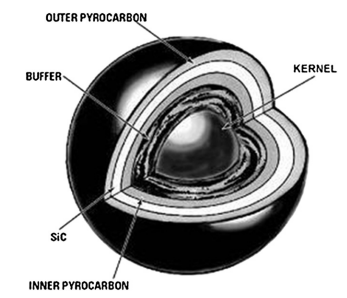
\includegraphics[width=0.9\linewidth]{figures/TRISO_diagram_Zhou_Tang.png}
            \caption{Layers from innermost to outermost: fuel kernel, buffer, Inner PyC, SiC,Outer PyC \cite{zhou_tang}.}
        \end{figure}
    \end{minipage}
    \hfill%
    \begin{minipage}[t]{0.45\linewidth}
        \begin{itemize}
            \item Common fuel for advanced reactors
            \item UCO fuel kernel radius 212.5 microns
            \item Outer PyC radius 427.5 microns
            \item Very good thermal properties, melting significantly higher than operational temperatures (quantify/source?)
            \item Encapsulates fission products well
            \item Either packed into graphite compacts or into spherical pebbles for PBRs
            \item TRISO modeling challenges
            \begin{itemize}
                \item Many surfaces per TRISO
                \item Many TRISOs per reactor
            \end{itemize}
        \end{itemize}
    \end{minipage}
\end{frame}

\begin{frame}{Virtual Test Bed Gas Cooled Microreactor}
    \begin{minipage}[t]{0.45\linewidth}
        \begin{itemize}
            \item Existing VTB GCMR simulations
            \begin{itemize}
                \item Preliminary multiphysics models: Griffin-BISON-SAM \cite{Abdelhameed-ANS-2022,Stauff-preliminary-applications-2021,Stauff-applications-2022}
                \item Dynamic multiphysics simulations: flow blockage and Reactivity Insertion Accident \cite{HF_MRs_ANL}
                \item Balance of plant 1D thermal hydraulic simulation \cite{Duchnowski_plant_balance_2022}
            \end{itemize}
            \item This work presents the first published OpenMC Model of the VTB GCMR
            \begin{itemize}
                \item Plans to add this infinte-assembly model to the VTB this summer
            \end{itemize}
            \item For a full core model, it will be prohibitively expensive to model every TRISO explicitly
        \end{itemize}
    \end{minipage}
    \hfill%
    \begin{minipage}[t]{0.45\linewidth}
        \begin{figure}
            \centering
            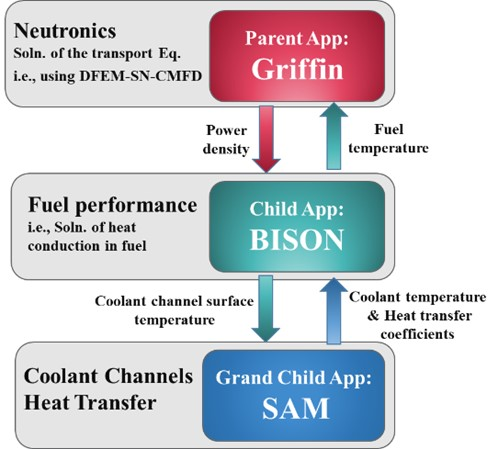
\includegraphics[width=0.9\linewidth]{figures/gcmr_preliminary_mutliapps.png}
            \caption{MultiApp hierarchy of preliminary work \cite{Abdelhameed-ANS-2022}.}
        \end{figure}
    \end{minipage}

\end{frame}

\begin{frame}{Research Goal}
    \begin{itemize}
        \item \textbf{What degree of explicitness is required to represent TRISO for a full-core model of the GCMR?}
        \item To answer this question, varying degrees of homogenization were used in an infinite-assembly depletion model, computing \kinf~as a function of burnup up to 29 GWday/tonne-U.
        \item Two homogenization strategies: ``\textbf{kernel only}'' and ``\textbf{full volume}''
        \item Kernel only homogenization takes all non-fuel layers of the TRISO and homogenizes them, by volume fraction, into the compacts' background graphite and then packs UCO kernels into the background
        \begin{itemize}
            \item Keeps the same original kernel positions as fully explicit
        \end{itemize}
        \item Full volume homogenization makes one material per compact with the all the individual components mixed by their original volume fraction in the fully explicit case.
        \item Comparing both homogenizations to the fully explicit case for the assembly model can be used as a basis for deciding how proceed with a full core model.
    \end{itemize}
\end{frame}

%%----------------------------------------------------------------------------%%
%% Section 2
%%----------------------------------------------------------------------------%%
\section{OpenMC Model}

\begin{frame}{OpenMC Model}
    \begin{minipage}[t]{0.2\linewidth}
        \begin{figure}
            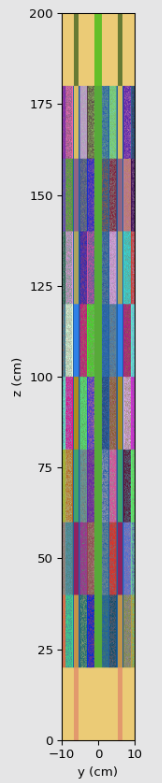
\includegraphics[height=0.7\textheight]{figures/yz_slice.png}
            \caption{YZ slice of reactor}
        \end{figure}
        \end{minipage}
    \begin{minipage}[t]{0.35\linewidth}
        \begin{figure}
            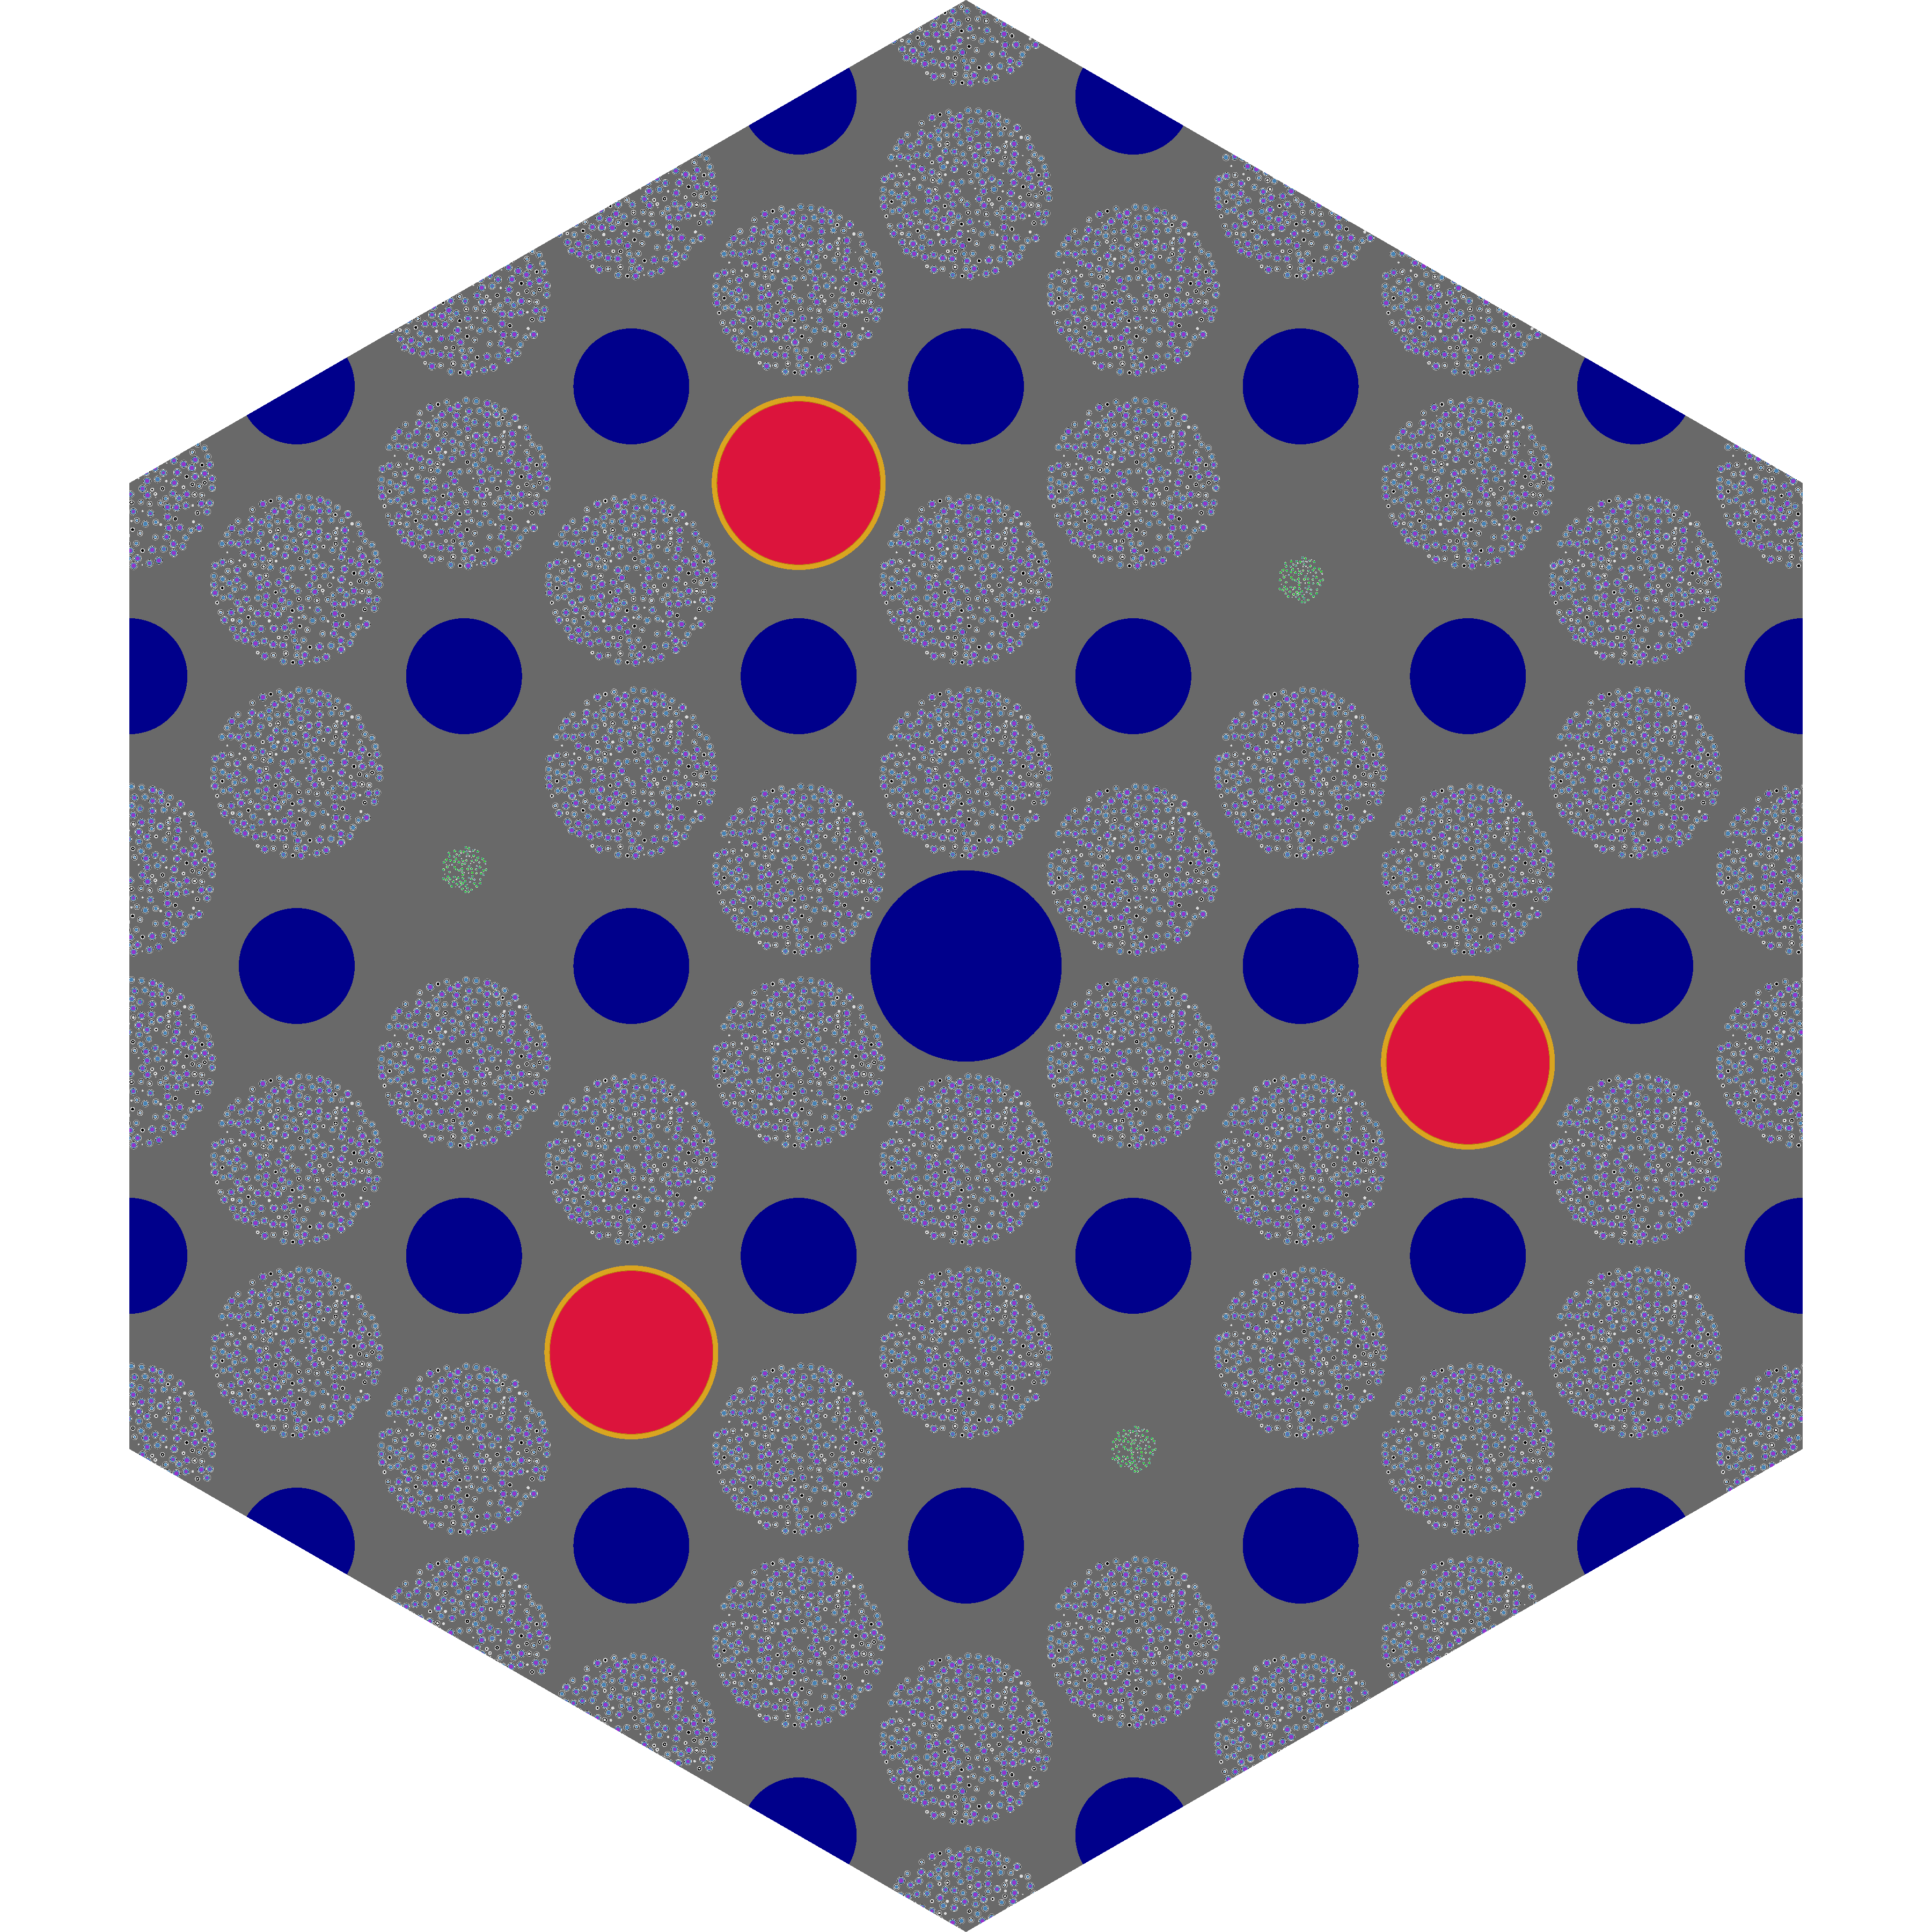
\includegraphics[height=0.7\textheight]{figures/gcmr_slice.png}
            \caption{XY slice of reactor}
        \end{figure}
    \end{minipage}
    \hfill%
    \begin{minipage}[t]{0.4\linewidth}
        \begin{itemize}
        \item 8 axial layers in the core, 2 axial layers per reflector
        \item pin pitch = 2cm 
        \item periodic BC on hexagonal boundary
        \item vacuum BC at top and bottom 
        \item Materials 
            \begin{itemize}
                \item gray = graphite
                \item blue = helium 
                \item red = YH2 moderator
                \item gold = FeCrAL envelope
                \item green = B4C poison spheres or B4C control rod
                \item purple dots = TRISO
                \item peach = upper/lower BeO reflectors
            \end{itemize}
        \end{itemize}
    \end{minipage}
\end{frame}


\begin{frame}{System Parameters}
    \begin{table}[h]
        \centering
        \begin{tabular}{|c|c|c|}
        \hline 
        & physical parameters & \\
        \hline
        fuel radius & poison radius & moderator radius  \\
        0.90 cm & 0.25 cm   & 0.843 cm  \\
        \hline
        control radius & coolant radius & FeCrAl thickness \\
        0.99 cm    & 0.60 cm & 0.05 cm \\
        \hline
        Cr coating thickness & fuel packing fraction & poison packing fraction \\
        0.007 cm & 0.4 -  & 0.25 - \\
        \hline
        reflector height & core height & enrichment \\
        \hline
        20 cm & 160 cm &  19.95\% \\
        \hline
        inlet temperature & outlet temperature & outlet pressure \\
        \hline
        873.15 K & 1133.65 K  & 7 MPa \\
        \hline
        \end{tabular}
        \vspace{-0.25cm}
        \label{tab:dimensions}
    \end{table}
\end{frame}

\begin{frame}{Depletion Simulation Parameters}

\end{frame}
%%----------------------------------------------------------------------------%%
%% Section 3
%%----------------------------------------------------------------------------%%
\section{Results and Discussion}

\begin{frame}{Eigenvalue comparisons across each spatial discretization}
    \begin{itemize}
        \item ratios vs burnup
    \end{itemize}
\end{frame}

\begin{frame}{Eigenvalue comparisons across each spatial discretization}
    \begin{itemize}
        \item average delta rhos
    \end{itemize}
\end{frame}

\begin{frame}{Eigenvalue comparisons across each spatial discretization}
    \begin{itemize}
        \item isotopics
    \end{itemize}
\end{frame}

%%----------------------------------------------------------------------------%%
%% Section 4
%%----------------------------------------------------------------------------%%
\section{Next Steps}
\begin{frame}{Two-layer TRISO Homogenization}
    \begin{itemize}
        \item
    \end{itemize}
\end{frame}

\begin{frame}{Full core model and multiphysics}
    \begin{itemize}
        \item
    \end{itemize}
\end{frame}


%%----------------------------------------------------------------------------%%`'
%% Bibliography
%%----------------------------------------------------------------------------%%

\begin{withoutheadline}
    \begin{frame}{Acknowledgements}
        \begin{itemize}
            \item The first author was supported in part by the US Nuclear Regulatory Commission's Graduate Fellowship Program administered by the University of Wisconsin-Madison.
            \item The Center for High Throughput Computing at the University of Wisconsin - Madison
            \item OpenMC team!
            \item Co-authors: Patrick Shriwise, Benjamin Lindley, and Paul P.H.~Wilson.
        \end{itemize}
        \begin{figure}[H]
            \centering
            
\includegraphics[height=0.3\textheight]{figures/openmc_logo.png}
        \end{figure}
        \begin{figure}[H]
            \centering
            
\includegraphics[height=0.3\textheight]{figures/CHTC.png}
        \end{figure}
    \end{frame}
\end{withoutheadline}

\begin{withoutheadline}
    \begin{frame}[allowframebreaks]{Bibliography}
        \printbibliography
    \end{frame}
\end{withoutheadline}

\begin{withoutheadline}
    \begin{frame}{Open Source Projects}
        \begin{itemize}
            \item OpenMC website: \href{https://openmc.org/}{https://openmc.org/}
            \item OpenMC repository: \href{https://github.com/openmc-dev/openmc}{https://github.com/openmc-dev/openmc}
            \item VTB: \href{https://mooseframework.inl.gov/virtual_test_bed/}{https://mooseframework.inl.gov/virtual\_test\_bed/}
            \item VTB repository: \href{https://github.com/idaholab/virtual_test_bed}{https://github.com/idaholab/virtual\_test\_bed}
            \item Add me on LinkedIn (\href{https://www.linkedin.com/in/lewisgross1296}{lewisgross1296}) and GitHub (\href{https://github.com/lewisgross1296}{lewisgross1296})!
        \end{itemize}
    \end{frame}
\end{withoutheadline}

\end{document}
